\section{Affine $n$-Space and Algebraic Sets}\label{section_1.2}

\begin{definition}
  Let $k$ be a field. We define  \textbf{affine $n$-space} over $k$ to be the
  cartesian product  $\A^n(k) = \underbrace{k \times \dots \times
  k}_{n\text{-times}}$. If the field $k$ is understood, we write  $\A^n$. We
  call the elements of  $\A^n(k)$ \textbf{affine points}. We call $\A^1(k)$ and
  $\A^2(k)$ the \textbf{affine line} and \textbf{affine plane} over $k$,
  respectively.
\end{definition}

\begin{definition}
  Let $k$ be a field, and let  $f \in k[x_1, \dots, x_n]$. We call an affine
  point $P \in \A^n(k)$ a \textbf{zero}, or \textbf{root} of $f$ if $f(P)=0$,
  where $P=(a_1, \dots, a_n)$, and $f(P)=f(a_1, \dots, a_n)$. We call
  the set of zeros of $f$, $V(f)$ the \textbf{hypersurface} defined by
  $f$. We call hypersurfaces in  $\A^2(k)$ \textbf{affine plane curves}.
  If $\deg{f}=1$, we call $V(f)$ a \textbf{hyperplane}. We call
  hypersurfaces in $\A^1(k)$ \textbf{lines}.
\end{definition}

\begin{example}\label{example_1.4}
  The following curves in figure \ref{figure_1.1} define algebraic sets.
  \begin{figure}[h]
    \centering
    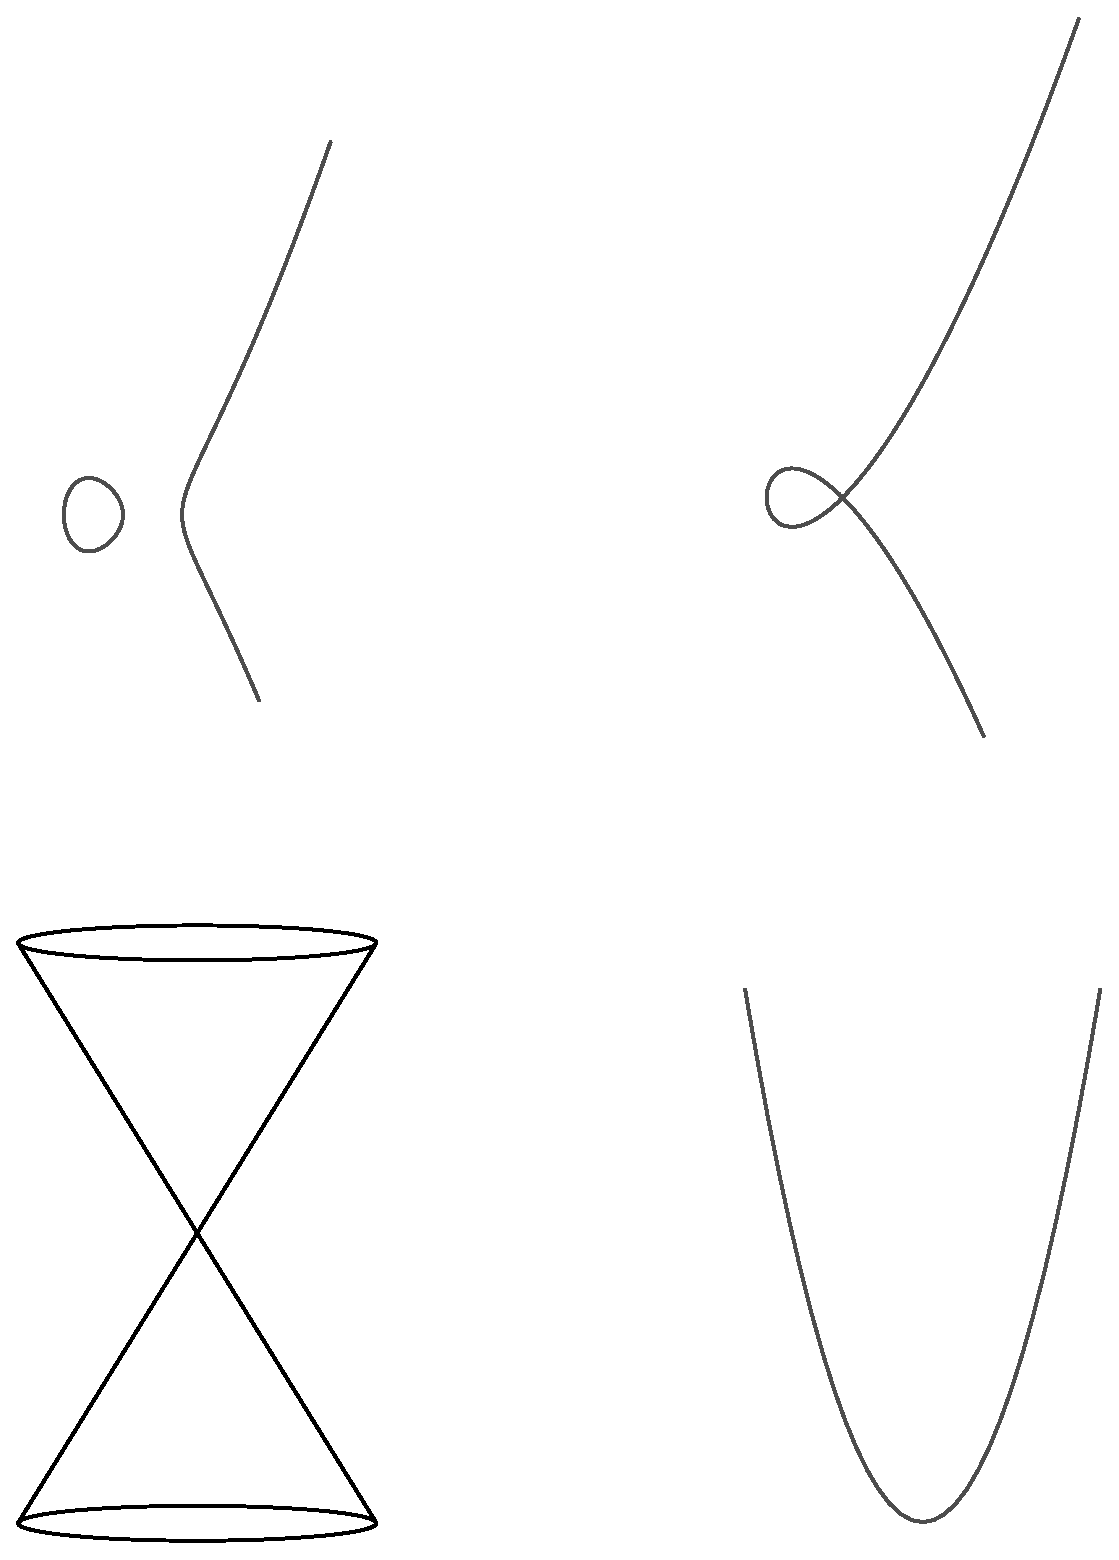
\includegraphics[scale=0.5]{Figures/chapter1/hyperplanes.eps}
    \caption{Affine Algebraic Sets in $\A^2(\R)$ and $\A^3(\R)$.}
    \label{figure_1.1}
  \end{figure}
\end{example}

\begin{definition}
  Let $k$ be a field, and $S$ any set of polynomials in $k[x_1, \dots, x_n]$.
  We define the \textbf{set of zeros} of $S$ to be the set  $V(S)=\{P \in
  \A^n(k) : f(P)=0 \text{ for all } f \in S\}$. We call a subset $X$ of
  $\A^n(k)$ an \textbf{affine algebraic set} if $X=V(S)$ for some set $S$ of
  polynomials.
\end{definition}
